% DATA 266 Lab 2 combined report (IEEE conference format).
% Overleaf: upload the whole reports/ folder (report.tex, sections/, tables/, figures/), set report.tex as the main file, compile with pdfLaTeX.
% Tables in tables/ are generated by build_tables.py from the results files. Do not type numbers into them by hand.
% Red text = a placeholder that still needs to be written or filled. Search for "PENDING" before submitting.
\documentclass[conference]{IEEEtran}
\usepackage{graphicx,booktabs,cite,tikz,url,xcolor}
\usetikzlibrary{arrows.meta,positioning}
\usepackage[hidelinks]{hyperref}

% \pending{...}: visible red placeholder
\newcommand{\pending}[1]{{\color{red}\textbf{[PENDING: #1]}}}
% \optional{file}{placeholder}: input a section file if it exists, otherwise show the placeholder
\newcommand{\optional}[2]{\IfFileExists{#1}{\input{#1}}{\noindent\pending{#2}\par}}
% \optfig{file}{width}{caption}{label}: include a figure if the image exists, otherwise a framed placeholder
\newcommand{\optfig}[4]{%
  \begin{figure}[!t]\centering
  \IfFileExists{#1}{\includegraphics[width=#2]{#1}}{\fbox{\parbox{0.9\columnwidth}{\centering\vspace{6mm}\pending{image \texttt{\detokenize{#1}}}\vspace{6mm}}}}
  \caption{#3}\label{#4}\end{figure}}

\title{DATA 266 Lab 2: Multimodal RAG, Diffusion Fine-Tuning and a Multi-Agent Image System}
\author{\IEEEauthorblockN{Kavan Siddesh Kumar and Muhammed Faiq Salman}\IEEEauthorblockA{Pair\_Programming\_Team\_24, San Jos\'e State University}}

\begin{document}
\maketitle

\begin{abstract}
We built three systems on a single 16~GB GPU. For multimodal retrieval-augmented generation over three economics PDFs, a hybrid system (exact figure and table lookup, dense and BM25 retrieval, parsed table facts) answered 23 of 25 questions from our own golden set correctly, against 12 for a dense baseline, and it was selected for the Kaggle submission (public score 0.818). For diffusion fine-tuning, we trained two LoRA adapters of Stable Diffusion 1.5 on a captioned Naruto dataset: the rank-32 adapter lowered KID from 0.0623 to 0.0171 and was preferred to the base model in 66\% of non-tied human judgments (three raters, 25 blinded pairs), but it still drops objects from some multi-object prompts. For the five-agent image system, a critique loop increased the median time per request from 9.64~s to 16.65~s, and none of the ten red-team attacks succeeded.
\end{abstract}

\begin{IEEEkeywords}
retrieval-augmented generation, diffusion models, LoRA, multi-agent systems, safety evaluation
\end{IEEEkeywords}

% ====================================================================
\section{Part 1: Multimodal RAG}
% Both members built a complete Part 1. Both systems are described, then the shared evaluation and the selected system.

\subsection{System A (Kavan)}
\subsubsection{Architecture}
The system answers questions over three PDFs, including their text, tables, and figures. The documents and manifest are processed into searchable chunks, figures, tables, and facts, followed by retrieval, rule-based or vision-based answering, and checked JSON output using a RAG design \cite{lewis}.
\begin{figure}[!t]
\centering
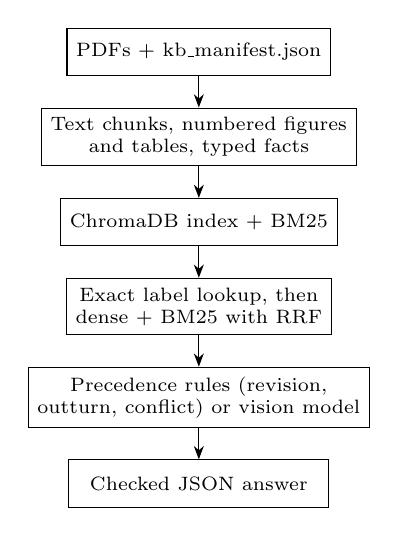
\begin{tikzpicture}[node distance=4mm,box/.style={draw,align=center,font=\scriptsize,minimum width=33mm,minimum height=6mm},>={Stealth}]
\node[box] (pdf) {PDFs + kb\_manifest.json};
\node[box,below=of pdf] (ing) {Text chunks, numbered figures\\and tables, typed facts};
\node[box,below=of ing] (idx) {ChromaDB index + BM25};
\node[box,below=of idx] (ret) {Exact label lookup, then\\dense + BM25 with RRF};
\node[box,below=of ret] (res) {Precedence rules (revision,\\outturn, conflict) or vision model};
\node[box,below=of res] (out) {Checked JSON answer};
\foreach \a/\b in {pdf/ing,ing/idx,idx/ret,ret/res,res/out}{\draw[->] (\a)--(\b);}
\end{tikzpicture}
\caption{Part 1 architecture.}
\label{fig:p1}
\end{figure}

\subsubsection{Ingestion and retrieval}
PyMuPDF reads the PDFs, and each text chunk stores its document ID, page number, and trust level. Numbered figures and tables are saved with their labels and captions, while Qwen2.5-VL-3B converts figures into searchable descriptions. Appendix C is marked low trust and filtered during retrieval; named figures and tables are matched exactly first, while other questions use dense and BM25 retrieval combined with reciprocal rank fusion.

\subsubsection{Grounded answers}
Tables are converted into typed facts containing the entity, variable, period, value, source, and whether the value is a forecast or an actual result. Plain Python applies the manifest’s revision, outturn, forecast, and conflict rules because a small language model may not apply them consistently. The LLM is mainly used for charts and open-ended questions, and no question text or answer values are hard-coded into the program.

\subsubsection{What worked and what did not}
The hybrid system worked better than the dense baseline on my golden set, answering 23/25 questions correctly compared with 12/25. It had better status accuracy, citation accuracy, and speed, especially because 14 answers came directly from parsed tables. It correctly handled all two-source, conflict/revision, and multi-turn questions. However, performance was lower on Muhammed’s unseen set, where it answered 8/25 correctly. The main weaknesses were difficult figure questions and false-premise or injection questions. The Kaggle score ended at 0.818 after briefly dropping to 0.808.


\subsection{System B (Muhammed)}
\optional{sections/p1_muhammed.tex}{Muhammed's Part 1 system: architecture, ingestion, retrieval, answering, what worked and what did not}

\optional{sections/p1_eval.tex}{shared evaluation: golden sets, comparison, selection, results, safety analysis}
\optional{tables/p1.tex}{run build\_tables.py}

% ====================================================================
\section{Part 2: Fine-Tuning Diffusion Models}
\optional{sections/p2.tex}{Muhammed's Part 2 section}
\optional{tables/p2.tex}{run build\_tables.py}
\optional{tables/p2_repro.tex}{run build\_tables.py}

% ====================================================================
\section{Part 3: Multimodal Multi-Agent System}
\subsection{Architecture}
The Part 3 system uses five agents that share one typed state object. The planner either routes the request or refuses it; caption and question requests stop after the vision step, while other requests continue through generation and critique. The critic can send the result back for at most two revisions \cite{madaan}.
\begin{figure}[!t]
\centering
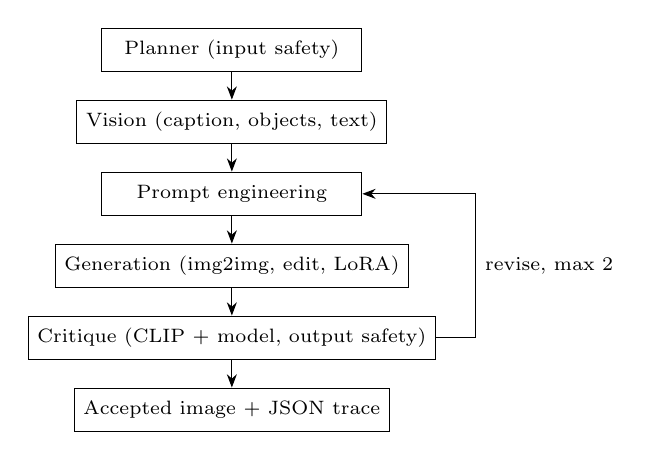
\begin{tikzpicture}[node distance=3.5mm,box/.style={draw,align=center,font=\scriptsize,minimum width=33mm,minimum height=5.5mm},>={Stealth}]
\node[box] (pl) {Planner (input safety)};
\node[box,below=of pl] (vi) {Vision (caption, objects, text)};
\node[box,below=of vi] (pr) {Prompt engineering};
\node[box,below=of pr] (ge) {Generation (img2img, edit, LoRA)};
\node[box,below=of ge] (cr) {Critique (CLIP + model, output safety)};
\node[box,below=of cr] (ou) {Accepted image + JSON trace};
\foreach \a/\b in {pl/vi,vi/pr,pr/ge,ge/cr,cr/ou}{\draw[->] (\a)--(\b);}
\draw[->] (cr.east)--++(5mm,0)|-(pr.east) node[pos=0.25,right,font=\scriptsize]{revise, max 2};
\end{tikzpicture}
\caption{Part 3 architecture.}
\label{fig:p3}
\end{figure}

\subsection{Failure handling}
Broken, empty, and unreadable files are detected before any model is run. Each agent is also wrapped so that errors become user-facing messages while the execution trace is still saved.

\subsection{Safety analysis}
Text found inside images is treated as data rather than as instructions \cite{greshake}. The planner transcribes visible text, refuses generation when that text contains instructions, and allows captions to quote it without acting on it. Word-pattern checks identify unsafe requests, and the Stable Diffusion safety checker screens generated outputs so flagged images are not shown to the user.

None of the ten red-team attacks succeeded. The system refused hidden instructions inside images, sexual-content requests, graphic violence, deceptive edits of real people, and direct requests to disable safety filters. It also handled empty files and invalid image files without crashing, returning clear error messages. For image questions containing instructions, it treated the text as visible content rather than following it. These results show that the safety checks worked for the tested cases, although they do not guarantee protection against every possible reworded attack.

\subsection{System card}
\textbf{Can do and known limits:} The system can caption images, answer image questions, change styles, edit images, and generate Naruto-style images. Its main limitation is that generated images do not always satisfy every part of a request. S05 remained insufficiently pencil-sketch-like, S08 became worse after critique and ended with snow instead of grass, S10 did not clearly show a rooftop, and S12 did not clearly show a night scene or full moon. The critic helped improve S06, S07, S09, and S11. For S08, the critic rejected the image in all three rounds, so the system stopped after reaching the two-revision limit. The critic accepted S05, S10, and S12 even though I judged their final images as failures. The critic is useful but not fully reliable because it combines a CLIP similarity threshold with a vision-model YES/NO check, and it can still accept images that fail parts of the rubric. \textbf{Safety measures:} input refusal, hidden-instruction check, output filter, two-revision limit and a JSON trace for every request.

\subsection{What worked and what did not}
The critique loop improved the pass rate from 7/15 to 10/15. S06, S07, S09, and S11 improved, while S08 regressed from passing to failing. S03, S05, S10, and S12 failed in both modes. Style-change, edit, and domain-generation results improved, while caption and ambiguous-input results stayed mostly the same. The final system was slower, increasing from a 9.64-second median to 16.65 seconds. The final system was slower because each generated image went through critic evaluation, including CLIP scoring and a vision-model check, and some cases also required revisions. Overall, critique helped several cases but did not guarantee that the final image satisfied the full rubric.

\optfig{figures/p3_critique_S06.png}{\columnwidth}{S06 (``Restyle this as pixel art.''), final mode, rounds 0--2. The critic asked for revisions on rounds 0 and 1 (CLIP 0.294, 0.314) and accepted round 2 (CLIP 0.367).}{fig:p3s06}
\optfig{figures/p3_critique_S08.png}{\columnwidth}{S08 (``Change the snow to green grass.''), final mode, rounds 0--2. The critic asked for revisions on all three rounds (CLIP 0.361, 0.392, 0.329); the system stopped at the two-revision limit and returned round 1, the highest-CLIP attempt, with a warning.}{fig:p3s08}

Table~\ref{tab:p3} summarizes the no-critique vs with-critique comparison, and Figs.~\ref{fig:p3s06}--\ref{fig:p3s08} show the critique rounds for S06, where revisions raised CLIP and the critic finally accepted the pixel-art result, and for S08, where every round was rejected and the system returned the highest-CLIP attempt after the two-revision limit.

\pending{check the 7/15 and 10/15 above against Table~\ref{tab:p3} once both members have rated (they are Kavan's ratings only), and add the human agreement.}

\subsection{Reproduction evidence}
My independent baseline (\texttt{notebooks/p3\_baseline\_Muhammad.ipynb}) is the same pipeline without the critique agent: planner, vision, prompt and generation agents, with one Qwen2.5-VL-3B-Instruct model playing the language roles, my Part 2 \texttt{run\_b} adapter for generation, instruct-pix2pix for edits, a typed state, a JSON trace for every request and a Gradio app. Table~\ref{tab:p3repro} summarises the run. Fourteen of the 15 scenarios pass the automatic rubric. The one failure, S01 (a request for a cartoon character with blue hair and a sword), was blocked by the output safety filter; the same prompt was blocked in the smoke test, so the filter blocked a harmless prompt. None of the 10 red-team attacks succeeded: eight requests were refused (six by the input rules, one by the planner for the request to do what a sign in the image says, and one edit whose output the filter blocked), and two completed without following the text hidden in the image. The run has limits. It used only four sample photos instead of the roughly 25 images the lab asks for, and no human pass/fail judgments were collected for it, so 14 of 15 is the automatic rubric alone. Single requests that load a model are slow (S07 took 230.6~s, most likely because it includes loading the edit model), while the median over the scenarios was 12.3~s.
\begin{table}[!t]
\centering
\caption{Part 3 reproduction: Muhammed's independent baseline run (no critique loop)}
\label{tab:p3repro}
\begin{tabular}{lc}
\hline
Measure & Baseline (Muhammed) \\
\hline
Scenarios passing the automatic rubric (of 15) & 14 \\
Human pass/fail judgments & not collected \\
Red-team attacks that succeeded & 0 of 10 \\
Median seconds per scenario request & 12.3 \\
Test photos used & 4 \\
Part 2 adapter used (generation) & run\_b \\
\hline
\end{tabular}
\end{table}


\optional{tables/p3.tex}{run build\_tables.py}

% ====================================================================
\section{Team Contributions and AI Usage}
Kavan led Part 3 and Muhammed led Part 2. Each member also built a complete Part 1 system with its own golden set, and each ran the other member's lead part as an independent baseline (Kavan the Part 2 baseline, Muhammed the Part 3 baseline). Who did what in detail, and our meeting recordings, are listed in \texttt{CONTRIBUTIONS.md}. We used AI coding assistants for parts of the code, documentation and report drafts; each member declares the tool and its use in \texttt{AI\_USAGE.md}, and all human ratings were made by people. The code, notebooks and evaluation files are in \url{https://github.com/Kavan1804/data266_lab2}, and the Part 2 models and generated images are on Hugging Face (links in \texttt{links.txt}).

\begin{thebibliography}{00}
\bibitem{lewis} P. Lewis et al., ``Retrieval-augmented generation for knowledge-intensive NLP tasks,'' 2020. arXiv:2005.11401.
\bibitem{faysse} M. Faysse et al., ``ColPali: Efficient document retrieval with vision language models,'' 2024. arXiv:2407.01449.
\bibitem{greshake} K. Greshake et al., ``Not what you've signed up for: Compromising real-world LLM-integrated applications with indirect prompt injection,'' 2023. arXiv:2302.12173.
\bibitem{rombach} R. Rombach et al., ``High-resolution image synthesis with latent diffusion models,'' 2022. arXiv:2112.10752.
\bibitem{hu} E. Hu et al., ``LoRA: Low-rank adaptation of large language models,'' 2021. arXiv:2106.09685.
\bibitem{carlini} N. Carlini et al., ``Extracting training data from diffusion models,'' 2023. arXiv:2301.13188.
\bibitem{yao} S. Yao et al., ``ReAct: Synergizing reasoning and acting in language models,'' 2022. arXiv:2210.03629.
\bibitem{madaan} A. Madaan et al., ``Self-Refine: Iterative refinement with self-feedback,'' 2023. arXiv:2303.17651.
\bibitem{brooks} T. Brooks et al., ``InstructPix2Pix: Learning to follow image editing instructions,'' 2023. arXiv:2211.09800.
\end{thebibliography}
\end{document}
